%% tags: boldmath; network; graph; edgeLabels; inOut; bentArrows
\PassOptionsToPackage{usenames,dvipsnames}{xcolor}
\documentclass[tikz,border=2]{standalone}
\usetikzlibrary{shadows,arrows,shapes,positioning,calc,backgrounds,fit}
%%
\definecolor{source}{HTML}{66C2A5}
\definecolor{sink}{HTML}{8DA0CB}
\definecolor{hub}{HTML}{FC8D62}
%%
% Define the layers to draw the diagram
\begin{document}
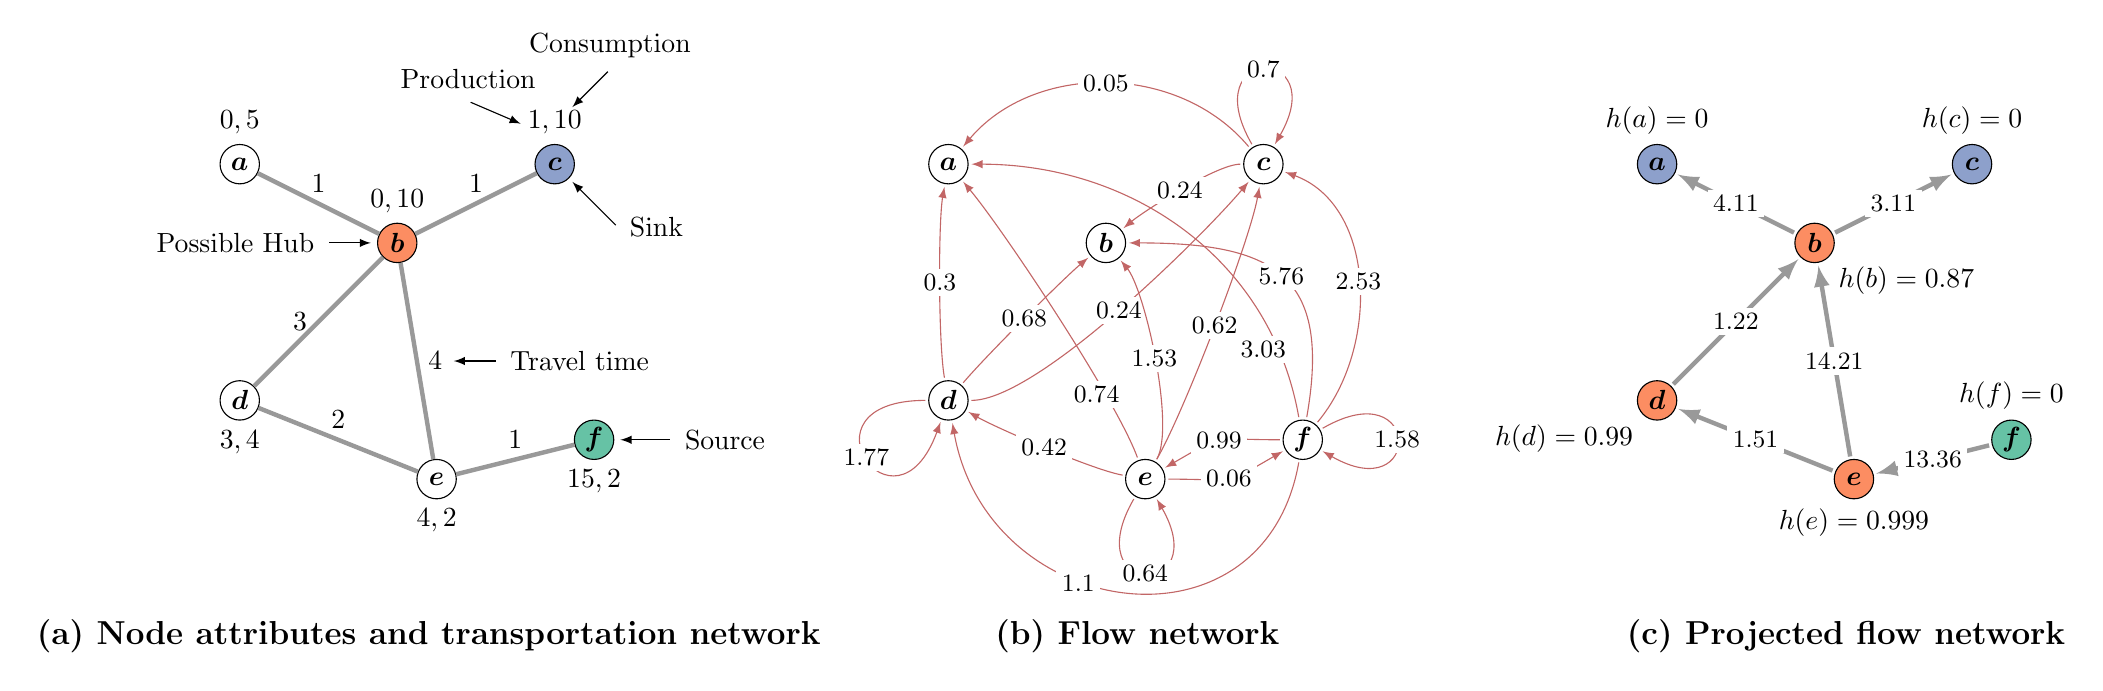
\begin{tikzpicture}
   [node distance=1cm,scale=2,
      vertex/.style={shape=circle,draw=black,inner sep=1pt,minimum
      size=.5cm,font=\boldmath},
lbl/.style={font=\small,inner sep=2pt},
trans/.style={ultra thick,black!40,text=black,midway},
gravity/.style={fill=white,font=\small,inner sep=2pt},
ledge/.style={thin,inner sep=2pt,>=latex, shorten >=1pt,
shorten <=1pt,looseness=.5},
gedge/.style={thin,inner sep=2pt,>=latex, shorten >=1pt,
shorten <=1pt,looseness=.5,red!60!black!60,text=black},
pedge/.style={trans,inner sep=2pt,>=latex, shorten >=1pt,
shorten <=1pt}]
%%
\newcommand{\xya}{(0,0)}
\newcommand{\xyb}{(1,-.5)}
\newcommand{\xyc}{(2,0)}
\newcommand{\xyd}{(0,-1.5)}
\newcommand{\xye}{(1.25,-2)}
\newcommand{\xyf}{(2.25,-1.75)}
%%
\begin{scope}
\node [font=\bfseries\large] at (1.2,-3) {(a) Node attributes and
transportation network};
\node (a) [vertex,label=above:{$0,5$}] at \xya {$a$};
\node (b) [vertex,label=above:{$0,10$},fill=hub] at \xyb {$b$};
\node (c) [vertex,label=above:{$1,10$},fill=sink] at \xyc {$c$};
\node (d) [vertex,label=below:{$3,4$}] at \xyd {$d$};
\node (e) [vertex,label=below:{$4,2$}] at \xye {$e$};
\node (f) [vertex,label=below:{$15,2$},fill=source] at \xyf {$f$};
%%
\draw[trans] (a) -- (b) node [trans,above] {$1$};
\draw[trans] (b) -- (c) node [trans,above] {$1$};
\draw[trans] (b) -- (d) node [trans,left] {$3$};
\draw[trans] (b) -- (e) node (tt) [trans,right] {$4$};
\draw[trans] (d) -- (e) node [trans,above] {$2$};
\draw[trans] (e) -- (f) node [trans,above] {$1$};
%%
%% labels
\draw[ledge,<-] ($(c)+(.1,.35)$) -- +(.25,.25) node [lbl,label=above:Consumption] {};
\draw[ledge,<-] ($(c)+(-.2,.25)$) -- +(-.35,.15) node [lbl,label=above:Production] {};
\draw[ledge,<-] ($(tt)+(.1,0)$) -- +(.3,0) node [lbl,label=right:Travel time] {};
\draw[ledge,<-] ($(c)+(.1,-.1)$) -- +(.3,-.3) node [lbl,label=right:Sink] {};
\draw[ledge,<-] ($(b)+(-.15,0)$) -- +(-.3,0) node [lbl,label=left:Possible Hub] {};
\draw[ledge,<-] ($(f)+(.15,0)$) -- +(.35,0) node [lbl,label=right:Source] {};
\end{scope}
%%
\begin{scope}[shift={(4.5cm,0cm)}]
\node [font=\bfseries\large] at (1.2,-3) {(b) Flow network};
\node (a) [vertex] at \xya {$a$};
\node (b) [vertex] at \xyb {$b$};
\node (c) [vertex] at \xyc {$c$};
\node (d) [vertex] at \xyd {$d$};
\node (e) [vertex] at \xye {$e$};
\node (f) [vertex] at \xyf {$f$};
%%
\path (c) edge[gedge,out=130,in=50,->,looseness=1] node[gravity] {$0.05$} (a);
\path (c) edge[gedge,out=180,in=40,->] node[gravity] {$0.24$} (b);
\path (c) edge[gedge,out=120,in=60,looseness=15,->] node[gravity] {$0.7$} (c);
\path (d) edge[gedge,out=100,in=260,->] node[gravity] {$0.3$} (a);
\path (d) edge[gedge,out=50,in=220,->] node[gravity] {$0.68$} (b);
\path (d) edge[gedge,out=0,in=230,->] node[gravity] {$0.24$} (c);
\path (d) edge[gedge,out=180,in=250,looseness=15,->] node[gravity] {$1.77$} (d);
\path (e) edge[gedge,out=110,in=-50,->] node[gravity,shift={(.5cm,-1cm)}] {$0.74$} (a);
\path (e) edge[gedge,out=60,in=-50,->] node[gravity] {$1.53$} (b);
\path (e) edge[gedge,out=60,in=-100,->] node[gravity] {$0.62$} (c);
\path (e) edge[gedge,out=170,in=-30,->] node[gravity] {$0.42$} (d);
\path (e) edge[gedge,out=240,in=-60,looseness=15,->] node[gravity] {$0.64$} (e);
\path (e) edge[gedge,out=0,in=210,looseness=1.5,->] node[gravity] {$0.06$} (f);
\path (f) edge[gedge,out=100,in=0,looseness=1,->]
node[gravity,shift={(1.0,-1.5)}] {$3.03$} (a);
\path (f) edge[gedge,out=80,in=0,looseness=1.5,->] node[gravity] {$5.76$} (b);
\path (f) edge[gedge,out=50,in=-20,looseness=1,->] node[gravity] {$2.53$} (c);
\path (f) edge[gedge,out=260,in=-80,looseness=1.5,->] node[gravity,shift={(-.6,0.1)}] {$1.1$} (d);
\path (f) edge[gedge,out=180,in=30,looseness=1.5,->] node[gravity] {$0.99$} (e);
\path (f) edge[gedge,out=30,in=-30,looseness=15,->] node[gravity] {$1.58$} (f);
\end{scope}
%%
\begin{scope}[shift={(9cm,0)}]
\node [font=\bfseries\large] at (1.2,-3) {(c) Projected flow network};
\node (a) [vertex,label=above:{$h(a)=0$},fill=sink] at \xya {$a$};
\node (b) [vertex,label=below right:{$h(b)=0.87$},fill=hub] at \xyb {$b$};
\node (c) [vertex,label=above:{$h(c)=0$},fill=sink] at \xyc {$c$};
\node (d) [vertex,label=below left:{$h(d)=0.99$},fill=hub] at \xyd {$d$};
\node (e) [vertex,label=below:{$h(e)=0.999$},fill=hub] at \xye {$e$};
\node (f) [vertex,label=above:{$h(f)=0$},fill=source] at \xyf {$f$};
%%
\path[pedge] (b) edge[pedge,->] node [gravity] {$4.11$} (a);
\path[pedge] (b) edge[pedge,->] node [gravity] {$3.11$} (c);
\path[pedge] (d) edge[pedge,->] node [gravity] {$1.22$} (b);
\path[pedge] (e) edge[pedge,->] node [gravity] {$1.51$} (d);
\path[pedge] (e) edge[pedge,->] node [gravity] {$14.21$} (b);
\path[pedge] (f) edge[pedge,->] node [gravity] {$13.36$} (e);
\end{scope}
\end{tikzpicture}
\end{document}
